
% Package imports.
\documentclass[10pt,landscape]{article}
\usepackage{multicol}
\usepackage{calc}
\usepackage{ifthen}
\usepackage[landscape, a4paper]{geometry}
\usepackage{amsmath,amsthm,amsfonts,amssymb}
\usepackage{color,graphicx,overpic}
\usepackage{hyperref}
\usepackage{subfigure}
\usepackage{caption}
\usepackage{wrapfig}
\usepackage{amssymb}
\usepackage{amsmath}
\usepackage{amsfonts}

\newenvironment{Figure}{\par\medskip\noindent\minipage{\linewidth}}
{\endminipage\par\medskip}

% Sets page margins.
\geometry{top=.2in,left=.2in,right=.2in,bottom=.2in}

% Turns off header and footer.
\pagestyle{empty}

% Redefine section commands to use less space and have smaller text.
% (Can change font size if `\tiny` is too small.
% See http://www.sascha-frank.com/latex-font-size.html as a reference.)
\makeatletter
\renewcommand{\section}{\@startsection{section}{1}{0mm}%
                                {-0.5ex plus -0.5ex minus -.2ex}%
                                {-0.5\baselineskip}%
                                {\normalfont\small\bfseries}}
\renewcommand{\subsection}{\@startsection{subsection}{2}{0mm}%
                                {-0.5ex plus -.5ex minus -.2ex}%
                                {-0.5\baselineskip}%
                                {\normalfont\small\bfseries}}
\renewcommand{\subsubsection}{\@startsection{subsubsection}{3}{0mm}%
                                {-0.5ex plus -.5ex minus -.2ex}%
                                {-0.5\baselineskip}%
                                {\normalfont\small\bfseries}}
\renewcommand{\paragraph}{\@startsection{paragraph}{4}{0mm}%
                                {-0.5ex plus -.5ex minus -.2ex}%
                                {-0.5\baselineskip}%
                                {\normalfont\small\bfseries}}

\makeatother

\usepackage[dvipsnames]{xcolor}
%TITLE Formating
\usepackage{titlesec}

\titlespacing*{\section}{0pt}{0pt}{0pt}%compact section titles
\titlespacing*{\subsection}{0pt}{0pt}{0pt}%compact subsection titles
\titlespacing*{\subsubsection}{0pt}{0pt}{0pt}%compact subsubsection titles

\titleformat{\section}
  {\normalfont\normalsize\bfseries\color{PineGreen}}{\makebox[18pt][l]{\thesection}}{0pt}{}[{\titlerule[1pt]}]
\titleformat{\subsection}
  {\normalfont\small\bfseries\color{OliveGreen}}{\makebox[18pt][l]{\thesubsection}}{5pt}{}
\titleformat{\subsubsection}
  {\normalfont\small\bfseries\color{TealBlue}}{\makebox[18pt][l]{\thesubsubsection}}{8pt}{}


\setcounter{section}{-1} %start with section 0
% % No section numbers.
% \setcounter{secnumdepth}{0}

% Minimal paragraph indenting and spacing.
\setlength{\parindent}{0pt}
\setlength{\parskip}{0pt plus 0.5ex}

% Canonical "init" statement.
\begin{document}

% Don't start new paragraphs if you don't need to.
\raggedright

% Font size.
\scriptsize

% Specifying number of columns.
% Asterisk "*" here to force the left-most column to fill first, then the next, ect.
% (Otherwise, all columns would fill down "equally".
\begin{multicols*}{4}

% Can play around with these as desired.
\setlength{\columnseprule}{0.25pt}
\setlength{\premulticols}{0.25pt}
\setlength{\postmulticols}{0.25pt}
\setlength{\multicolsep}{0.25pt}
\setlength{\columnsep}{0.25pt}

% This is the "magic" pandoc variable. (This is where your Rmarkdown document is inserted.)
% insert section 
\input{Chapters/Lesson1}

\section{Linear regression}
\textbf{Linear Model}: $f(x) = \Tilde{w}^T\Tilde{x}+w_0 = w^Tx, x \in \mathbb{R}^d, y \in \mathbb{R}^n$\\
    Error Measurement: $\hat{w}= \underset{f \in w}{\text{argmin }}||y-Xw||^2$\\
    $\nabla_w||y-Xw||^2 = 2X^T(Xw-y)$, $O(nd)$, 
    \textbf{Closed Form Sol}: $\hat{w}= (X^TX)^\dagger X^Ty$, $O(nd^2)$, $n > d$: unique, $n < d$: exist 
%     via geometrical argument:
% 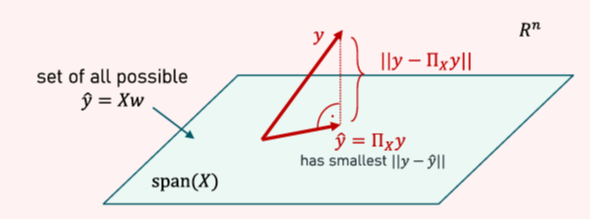
\includegraphics[width=0.6\linewidth]{pics/figure1.PNG}
    
\textbf{Huber loss }:
%\begin{equation}
    %L_{\delta}= 
    %\left\{\begin{matrix}
        % \frac{1}{2}(y - \hat{y})^{2} & if \left | (y - \hat{y})%  \right | < \delta\\
%        \delta ((y - \hat{y}) - \frac1 2 \delta) & otherwise
%   \end{matrix}\right
%\end{equation}
ignore outliers by giving less penalties
    
\begin{tabular}{c}
    $L_{\delta}(y, f(x))$ =
    $\begin{cases} 
        0.5 * (y - f(x))^2, \quad |y - f(x)| \leq \delta \\ 
        \delta * (|y - f(x)| - 0.5 * \delta),   \quad otherwise
    \end{cases}$
    \vspace{-0.3cm}
\end{tabular}


\section{Optimization}
\textbf{Gradient descent update (steepest descent direction)}:
$w^{t+1} = w^t - \eta\nabla_w L(w^t)$
Maximal Stepsize: $\eta \leq \frac{2}{\lambda_{max}}$\quad  $\lambda$: Eigenvalues of $X^TX$ \\
Fastest Stepsize: $\eta = \frac{2}{\lambda_\mathrm{min}+\lambda_\mathrm{max}}$\\
\textbf{Speeding up gradient descent}: 
Momentum (prevent oscillation) $w^{t+1} - w^{t} = \alpha(w^t - w^{t-1}) - \eta\nabla L(w^t)$ \\
Adaptive Methods (AdaGrad, RMSProp, Adam etc.) $w^{t+1}_i = w^t_i - \frac{\eta}{\sqrt{{previouschange}_i + \gamma}}\frac{\partial L}{\partial w_i}(w^t)$ \\
%\textbf{Stochastic Gradient Descent: }
%compute gradients using random subset of points instead of all points\\
\textbf{Convexity}:Guarantees \textcolor{blue}{local = global minimum}\\

1. iff $L(\lambda w + (1-\lambda)v) \leq \lambda L(w) + (1-\lambda)L(v)$;
2. or iff $L(v) \geq L(w) + \nabla L(w)^T(v-w)$ 
3. or iff $\nabla^2L(w)$ positive semi-definite

%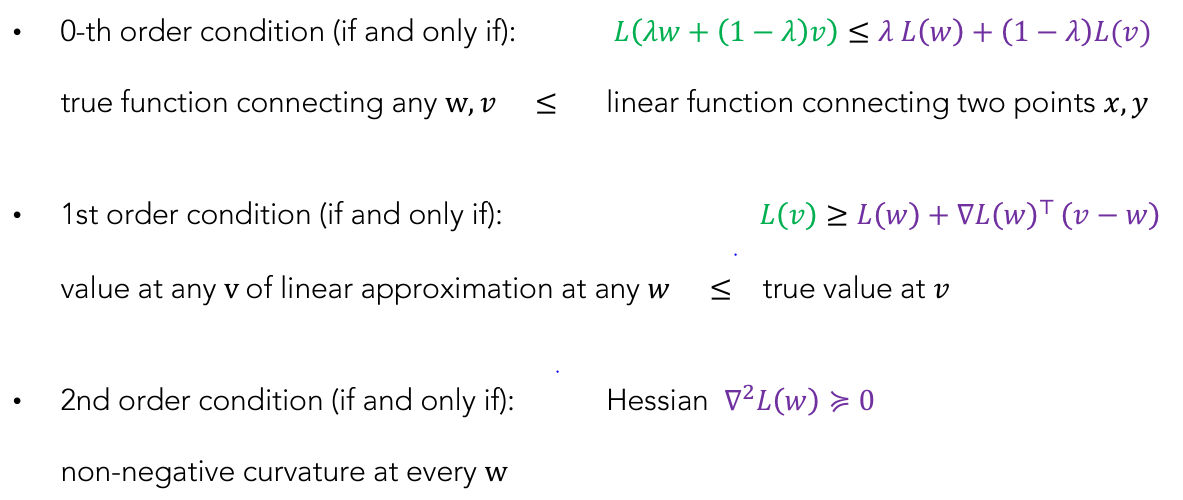
\includegraphics[width=0.8\linewidth]{pics/figure2.PNG}\\
Operation for \textbf{preserving} Convexity:\  if $f, g$ are convex \\
- $\alpha f + \beta g \ \ \forall \alpha, \beta \geq 0$ \qquad
- $h(x) = max\{f(x), g(x)\}$

$g$ affine $f$ convex \textbf{or} $f$ non-decreasing and $g$  conv:
$f \circ g$ 


\textbf{Strong convex}:
if $\exists m>0, L(w) - \frac{m}{2} ||w||^2$ is convex \textbf{or} $\nabla^2 L(w) > m\mathbf{I}^2$

For linear regression: Only \textcolor{blue}{one unique} global minimum if $\nabla^2_XL(w)=X^TX$ p.d.; many minima if p.s.d.\\
\textbf{Effects of increasing sample size}:
Let $d$ = sample dimension, $n$ = sample number: \\
For noiseless case: square loss decreases when fixing $d$ and increasing $n$; For noisy case, square increase and then decreases after $n \geq d$ (forced to fit the noise)

\section{Model selection}
\textbf{Prediction Error vs. Estimation Error}:
$R(f) = \mathbb{E}_{(x,y)}[(y - \hat{f}_D(x))^2] = \textcolor{blue}{\mathbb{E}_{x}[(f^{*}(x)-\bar{f}(x))^2]} + \mathbb{E}_{x}[(Var[\hat{f}_D(x)]] + \textcolor{orange}{\epsilon^2}$ average prediction / generalization error = \textcolor{blue}{$bias^2$} + \textcolor{orange}{irreducible noise} 
\textbf{cross validation}: \\
- (Typically choose K = 5 or 10 in practice)
- Fit the model and compute the validation error on each fold k  
- Average the cross-validation error over K folds  
- Select the model with lowest CV error 
- Model training and evaluation(training set $\&$ test set)

\textbf{LOOCV}:
if K very large, e.g. $K=|D_{rest}|$, we can get best approximation of
$M_\varPhi\{D_{rest}\}$. 

Problem: Computationally intensive. 


 \section{Regularization}
\textbf{Bias of method M}: \\
distance of average model $\bar{f} = \frac{1}{K}\sum_{k=1}^{K}\hat{f}_k$ to the ground truth $f^{*}(x)$: $\mathbb{E}_{x}(f^{*}(x)-\hat{f}(x))^2$ \\
\textbf{Variance of method M}:
average distance of individual models to average model $\mathbb{E}_{x}[\sum_{k=1}^{K}(f^{*}(x)-\hat{f}(x))^2]$ \\
\textbf{Bias variance decomposition and trade-off}: \\
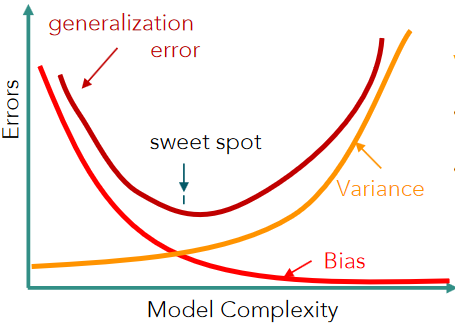
\includegraphics[width=0.35\linewidth]{pics/figure3.PNG} 
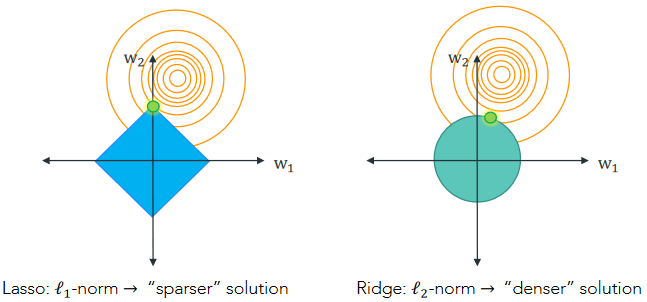
\includegraphics[width=0.6\linewidth]{pics/figure4.PNG}\\
\textbf{Geometric insight of lasso and ridge regression}
\textbf{Model complexity reflected in norms}: \\
- The larger the norm, the larger the space in $\mathbb{R}$ you use $\rightarrow$ higher model complexity \\
- Fitting noise often causes norm/model complexity to increase by using more unnecessary features\\
\textbf{Lasso regression}: (convex)
only use a few of these feature, encourage sparsity via limiting $l_1$-norm. (manually limiting the polynomial degree), \textbf{NO} close form $(\hat{w}^{\lambda}_i) = sign(\hat{w}_i)max(0, |(\hat{w}_i)| - \lambda))$ \\
The problem formulation: $\arg \min_{w}$ $||y - \phi w||^2$ s.t. $||w||_1 \leq R \rightarrow \arg \min_{w}$ $||y - \phi w||^2 + \lambda ||w||_1$\\
\textbf{Ridge regression}
The problem formulation: same as above except $||w||_2^2$ \quad\quad strict convex\\ 

Closed-form solution (find stationary point): $\hat{w_{\lambda}} = (X^TX + \lambda I)^{-1}X^Ty$ (or use the gradient methods) \\

\textbf{Cross-validation for $\lambda$ selection}\\
- Given a choice of features $\lambda$; - Find the best fit model for each fold: $\hat{f}^{\lambda}_k = M_{\lambda}(D_k) = \arg \min_{f} L_0(f;D_k) + \lambda ||f||$; - Others procedure same as normal CV


\section{Classification}
\textbf{Average classification (generalization) error}\\
$R(\hat{f}) = \mathbb{E}_{x,y}\mathbb{I}_{y \neq sign \hat{f}(x)}$ (the surrogate loss function is neither convex nor continuous, so it could not be used for minimizing training error!) \\
\textbf{Convexify the surrogate losses}\\
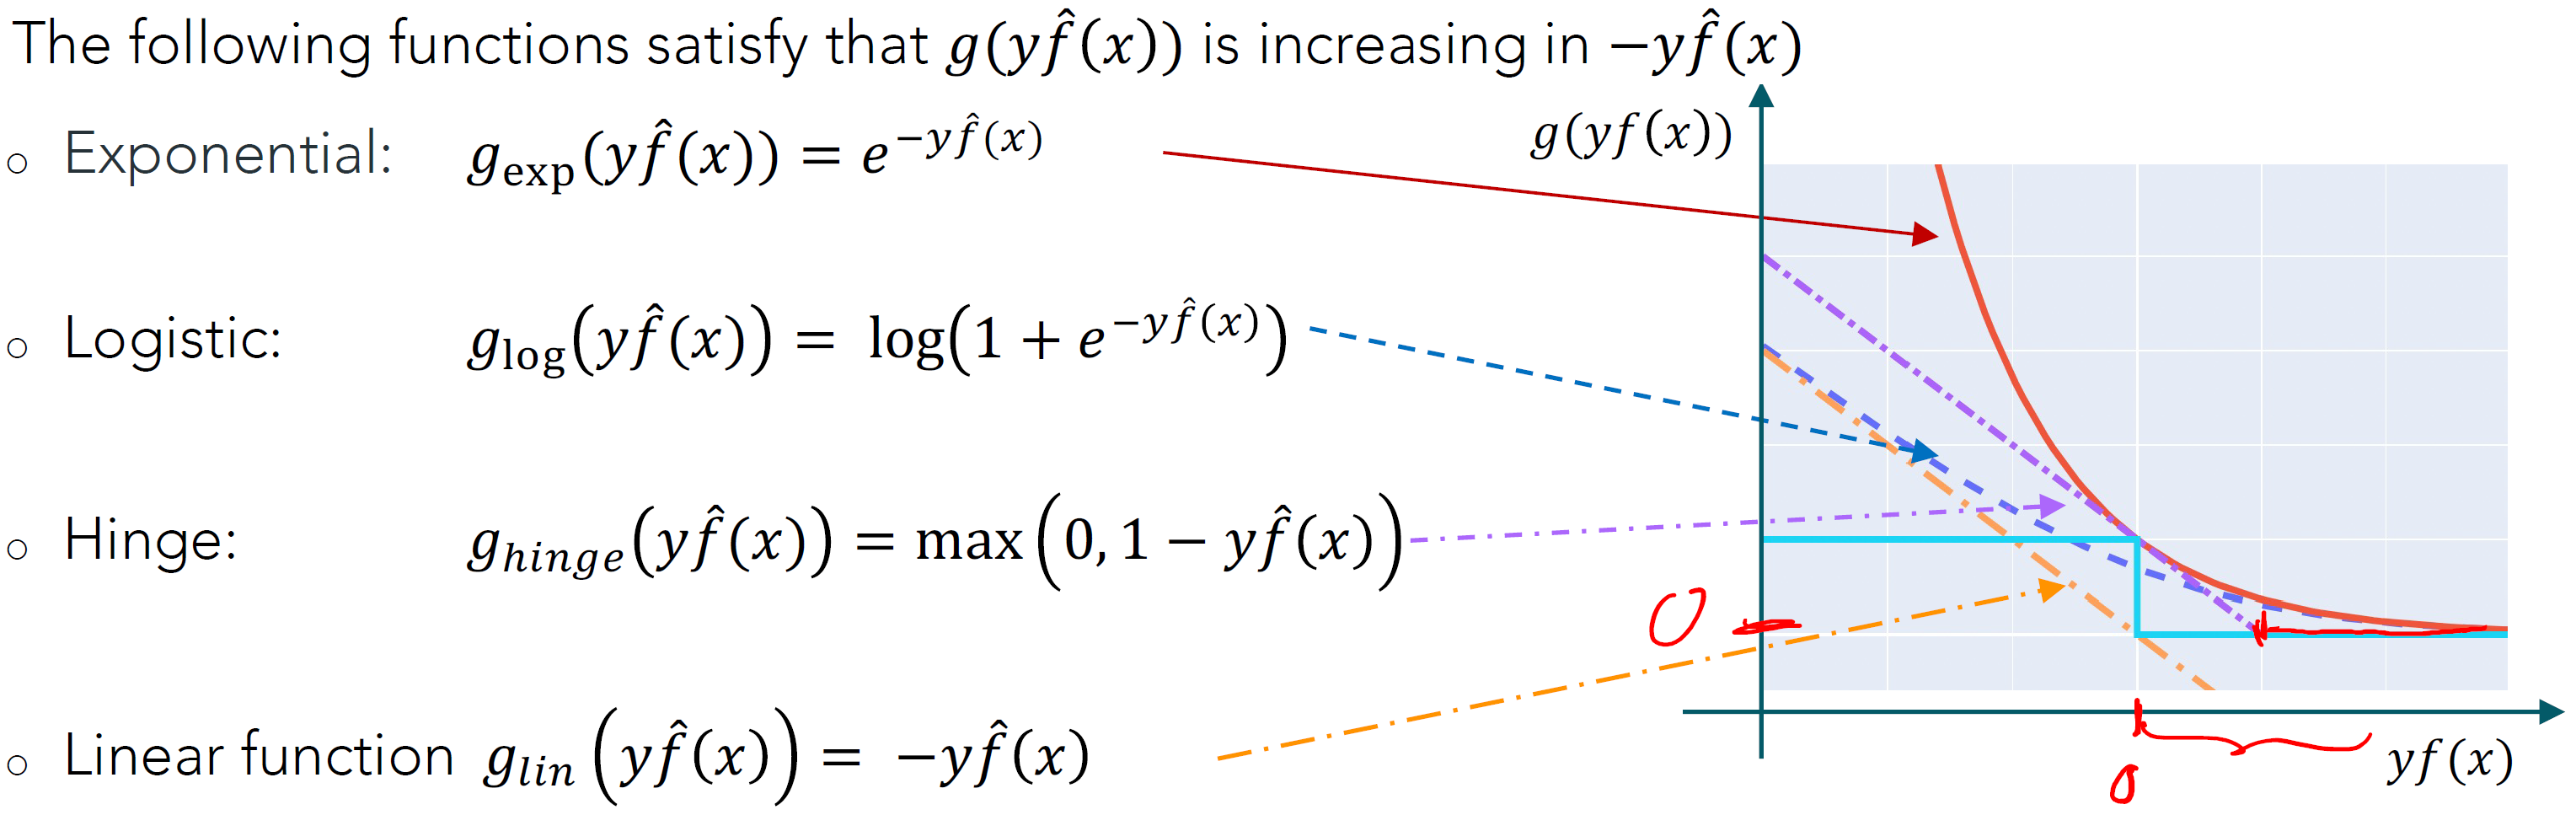
\includegraphics[width=\linewidth]{pics/figure5.PNG} 
\textbf{Logistic loss}: binary classification\\
$\ell_{log}(\hat{f}(x), y) = log(1 + e^{-y\hat{f}(x)}) = -log(Prob(Y=y|x)$ (condi. log-likeli.  param. by $\hat{f}(x) = (\hat{f}_1(x), \cdots, \hat{f}_k(x))$ via $p_i = softmax(\bar{f}_i) = \frac{exp(\alpha \Bar{f_i})}{ \sum_{j=1}^K exp(\alpha \Bar{f_j})}, \alpha > 0$) \\
\textbf{Cross-entropy loss}: multi-class classification see 10.3
\textbf{Maximum-Margin and SVM}: \\
Motivation: for linearly separable data, \textbf{no unique solution} for the training loss by using the logistic loss. \\
General formulation of the optimization problem: $w_{MM} = \arg \max_{||w||_2 = 1} margin(w)$ where margin$(w)=\min_{i} y_i\langle  w , x_i \rangle$  \\
\textbf{Soft-Margin SVM} \\
If data is not linearly separable (constraints that allow some "slack" in the constraint):\\
%\begin{equation}
$\min_{w,\xi} \frac{1}{2}||w||^2 + \lambda\sum_{i} \xi_{i}$ 
%\end{equation}
s.t. ${y_i}{w^T}{x_i} \geq 1 - \xi_{i}, {\xi_{i} \geq 0}$ for all i = 1, ...., n\\
converted to ($l_2$ penalized hinge loss):\\
%\begin{equation}
$\min_{w} \frac{1}{2}||w||^2 + \lambda\sum_{i} \max(0, 1-{y_i}{w^T}{x_i})$\\
%\end{equation}

\textbf{Area under the ROC (AUROC)}:\\
Ideal curve: higher TPR (y-axis) \& lower FPR (x-axis)\\
\textbf{F1-score}:$F_1 score = \frac{2}{\frac{1}{recall} + \frac{1}{precision}}$ (Why not average? For both recall and precision to be large) \\
\textbf{Accuracy:} $\operatorname{Acc}(y,\hat{y})=\frac{1}{n_{\mathrm{samples}}}\sum_i 1(\hat{y}_i=y_i)$ \\
\textbf{Recall \& Precision}
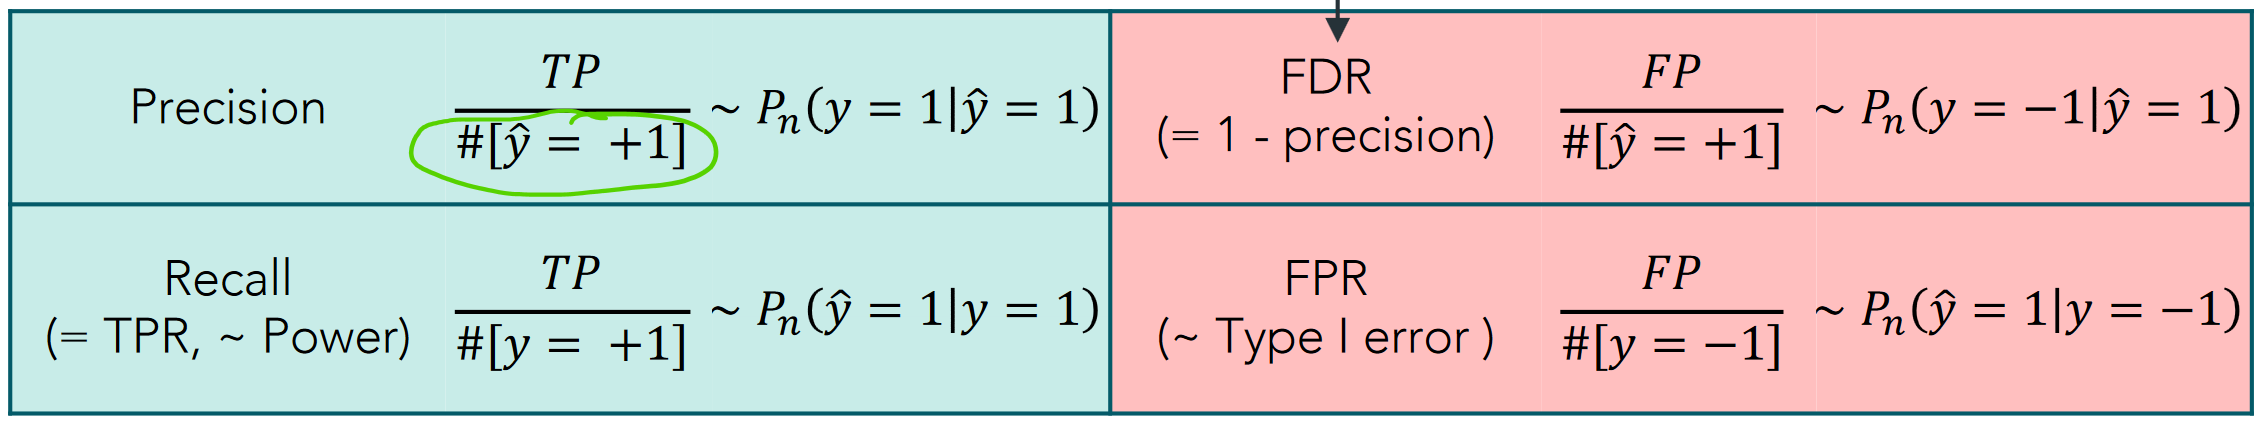
\includegraphics[width=\linewidth]{pics/figure6.PNG} \\
\textbf{Other metrics in practice}: \\
1. Worst group error (related to group fairness);\\
2. Advesarial pertubations (robustness againts data transformations);\qquad
3. Distribution shifts on the inputs (same label but data looks different)






\section{Kernel Methods}
Motivation: solve issue of feature explosion (extreme dimensionality of data): \#training data= n + m-th degree polynomial features + $ \phi(x) \in R^d$  + $ x \in R^p$

\textbf{Dim of feature map $\phi(x)$:} $p = (d+m, m) = \frac{(d+m)!}{m!d!}$ $O(d^m) = f(d)$ and $O(m^d) = f(m)$, size of total training data = np

\textbf{Kernel trick}
Step I: global minimizer $\hat{w} = \arg \min_{w \in R^p} \frac{1}{n} \sum^{n}_{i=1}l(y_i, f_w(x_i))$ has the form $\hat{w} = {\phi}^T\hat{\alpha}$ with $\hat{\alpha} \in R^n$ so that $\hat{f}(x) = \sum^{n}_{i=1}\hat{\alpha}_i \langle  \phi(x_i), \phi(x) \rangle$ and where $\hat{\alpha}$ only depends on $x_i$ via inner products $\langle  \phi(x_i) , \phi(x_j) \rangle$ for $i, j = 1, ..., n$ (save memory $O(n{d^m}) \rightarrow O(n^2)$ - kernel matrix)\\
Step II: $\langle \phi(x), \phi(z) \rangle = (1 + \langle x,z \rangle)^m$ Efficient computation for the inner product of kernel function (from $O(p)\sim O(d^m)$ to $O(d+m)$) (kern.matr. $K$ has $n^2$ kernels comput. complex. $O((d+m)n^2)$)\\

\textbf{Kernelized regression}:
%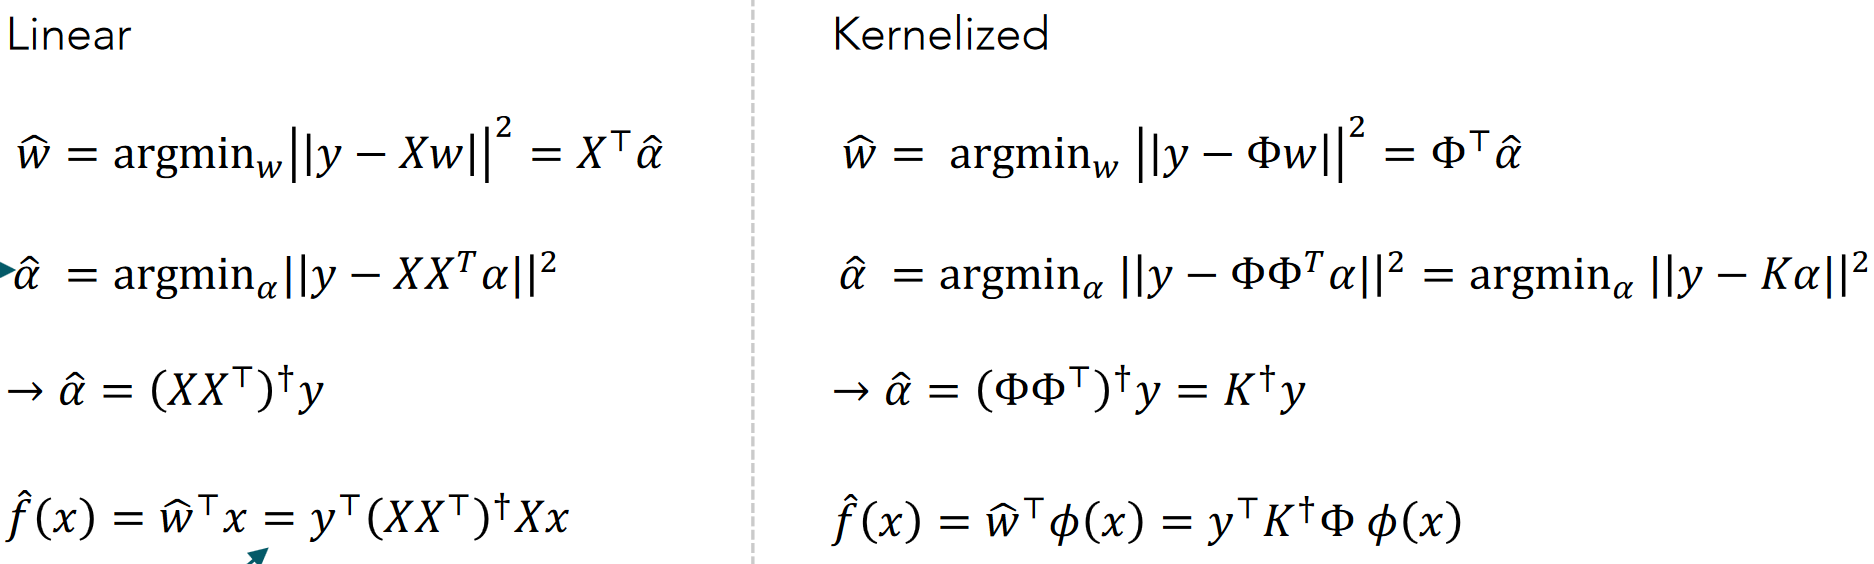
\includegraphics[width=\linewidth]{pics/figure7.PNG} \\
$\hat{w} = \arg \min_w ||y-\phi w||^2 = \phi^T \hat{\alpha}$ where $\hat{\alpha} = \arg \min_{\alpha}||y-\phi\phi^T\alpha||^2 = \arg \min_{\alpha} ||y-K\alpha||^2$\\
\textbf{Kernelized loss with ridge regularization}:
$\arg \min_{\alpha \in \mathbb{R}^n} ||y - K\alpha||^2 + \lambda {\alpha^T}K\alpha$\\
\textbf{Proof of kernel trick}:\\
Kernel trick can limit search from $R^d$ to $S$ ($S = span \{\phi(x_1), ..., \phi(x_n)\}$) \\
\textbf{Marcel's Theorem}: For kernels $k:X \times X \rightarrow R$ on a compact domain $X \in R^d$, $\exists$ sequence $\{\mu_j\}^{\infty}_{j=1}$ and basis $\{\phi_j\}^{\infty}_{j=1}$ of $L_2(X)$ (a sequence of functions) such that $k(x, y) = \sum^{\infty}_{j=1}\mu_j \phi_j(x)\phi_j(y) = \langle  \tilde{\phi}(x_j) , \tilde{\phi}(y_j) \rangle$ 

\textbf{Valid kernels} symmetric + psd: 
$min\{x, z\}$, 
const. $> 0$,  
$x^Tx'$, 
$|A \cap B|$, 
RBF kernels: $k(x, z) = e^{-\frac{||x-z||^{\alpha}}{\tau}}$, $\tau \downarrow$ overfit
(Gaussian: $\alpha = 2$\quad Laplacian: $\alpha = 1$)\\
\textbf{k-Nearest Neighbor}: can be kernelized\\
1. Sensitive to initialization (using cross-validation for choosing k);\quad
2. becomes erratic in high dimensions (all points become far);\quad 
3. needs large n to perform well but computation $O(nd)$, can reduce to $O(n^{\rho}), \rho < 1$ if allowing some error probability\\
\textbf{Decision trees}:
Leaf nodes of a binary tree. \textbf{But}
- can easily overfit to noise; - inaccurate as the greedy method









\section{Neural Networks}
Motivation: train feature maps $\phi$ and weights $w$ (generally non-convex, initialization matter) $w^* = \arg \min_{w, \textcolor{blue}{\theta_j}} \sum^n_{i=1}l(y_i; \sum^m_{j=1}{w_j}{\phi(x_i;\textcolor{blue}{\theta_j})})$

\textbf{Activation functions}
1. Identity; 2. Sigmoid: $\frac{1}{1+exp(-z)}$; 3. Tanh: $\frac{exp(z)-exp(-z)}{exp(z)+exp(-z)}$; 4. ReLU: $max(0, z)$ 

%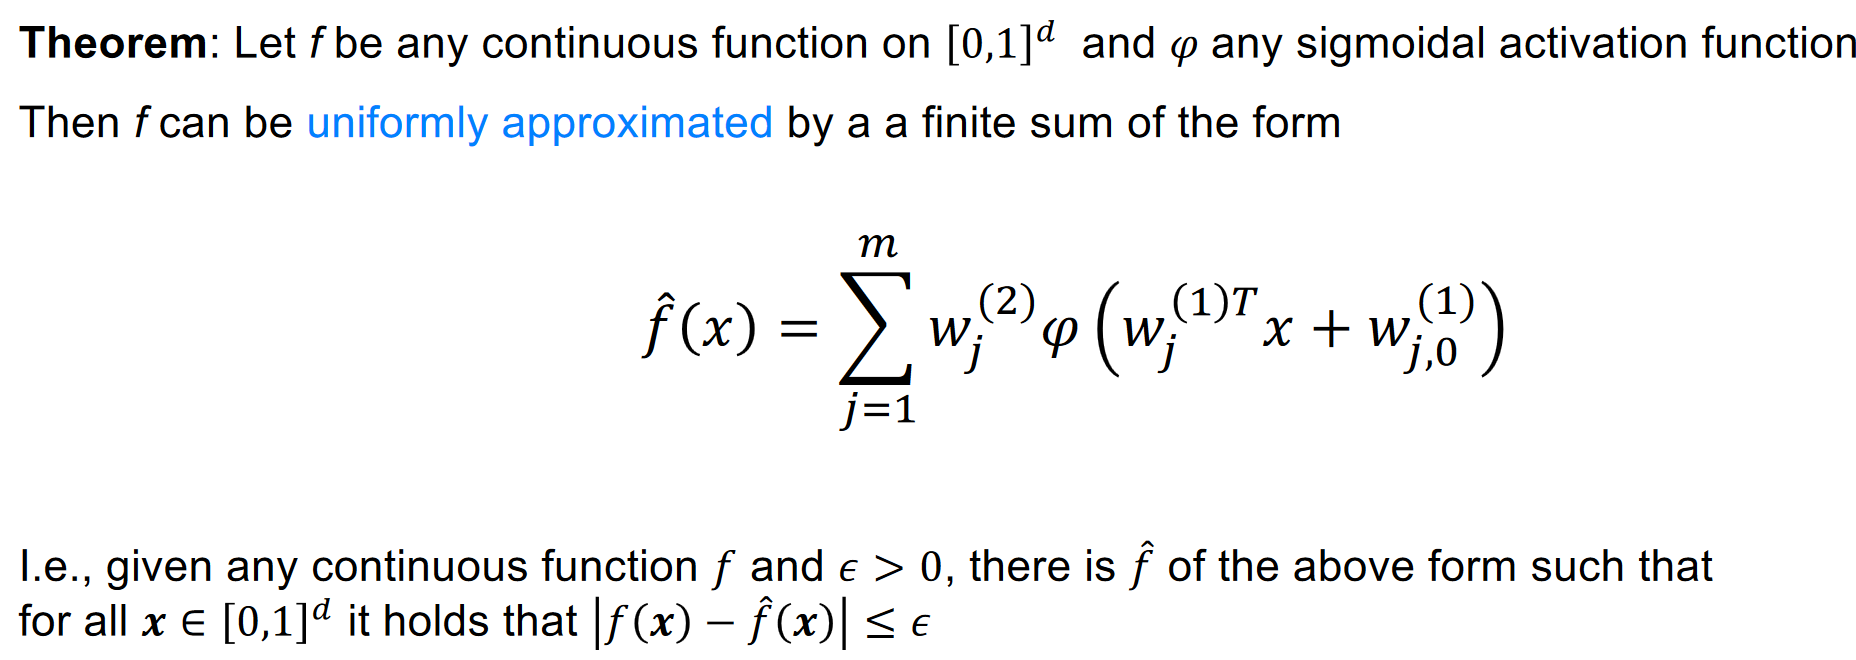
\includegraphics[width=\linewidth]{pics/figure8.PNG}
\textbf{Derivative of activation functions} \\
1. Sigmoid $\phi'(z)$ = $(1-\phi(z))\phi(z)$; 2. ReLU $\phi'(z) = 1$ if $z>0$; $0$ if $z<0$ (not differential at z=0, manually define derivative at 0 is 0)\\
\textbf{Backpropagation}
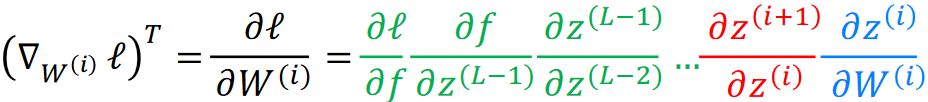
\includegraphics[width=\linewidth]{pics/figure9.PNG}
or it can rewrite into Matrix form:\\
$\nabla_{W^{(i)}}l = \delta^{(i)}\nu^{(i-1)T}$ where  error signal: \\ $\delta^{(i)} = 
\begin{cases}
\nabla_f l&, \text{output layer}\\
\varphi'(z^{(i)}) \odot (W^{(i+1)T}\delta^{(i+1)})&, \text{hidden layer}
\end{cases}$\\
and $\nu^{(i)} = \varphi(W^{(i)}\nu^{(i-1)})$\\
\textbf{Potential Issue}
Exploding or vanishing gradient (solve by using certain activation function, e.g. ReLU or keeping the magnitude of $\nu^{(i)}$)\\
\textbf{Initializing weights}
Goal: Keep variance of weights approximately constant across layers to avoid vani. and explod. grad. 
\textbf{Random initialization} 
Glorot ($tanh$), He (ReLU)
\textbf{Avoid overfitting}
Regularization (weight decay); Early stopping; Dropout p (=Pr(remain), test: $\sigma(W \times p)$)



\section{Convolutional Networks}
\textbf{CNN vs ANN}:\\
- Invariance to the augumentation of the training set\\
- Fewer parameters (parameters sharing in CNN)\\
- The weights can still be optimized via backprop.\\
\textbf{Batch normalization}:\\
1. Use on the mini-batch;\ 
2. Reduces internal covariate shift;\ 
3. Enables larger learning rates;\ 
4. Has regularizing effect
5. Solve vani./expl. grad.\\ 
1. Normalize each point with mini-batch mean and variance $\hat{x}_t = \frac{x_t-\mu_s}{\sqrt{\sigma_s^2+\epsilon}}$; 2. Scale and shift with 2 learnable parameters $\Tilde{x_t} = \gamma \hat{x_t} + \beta$
%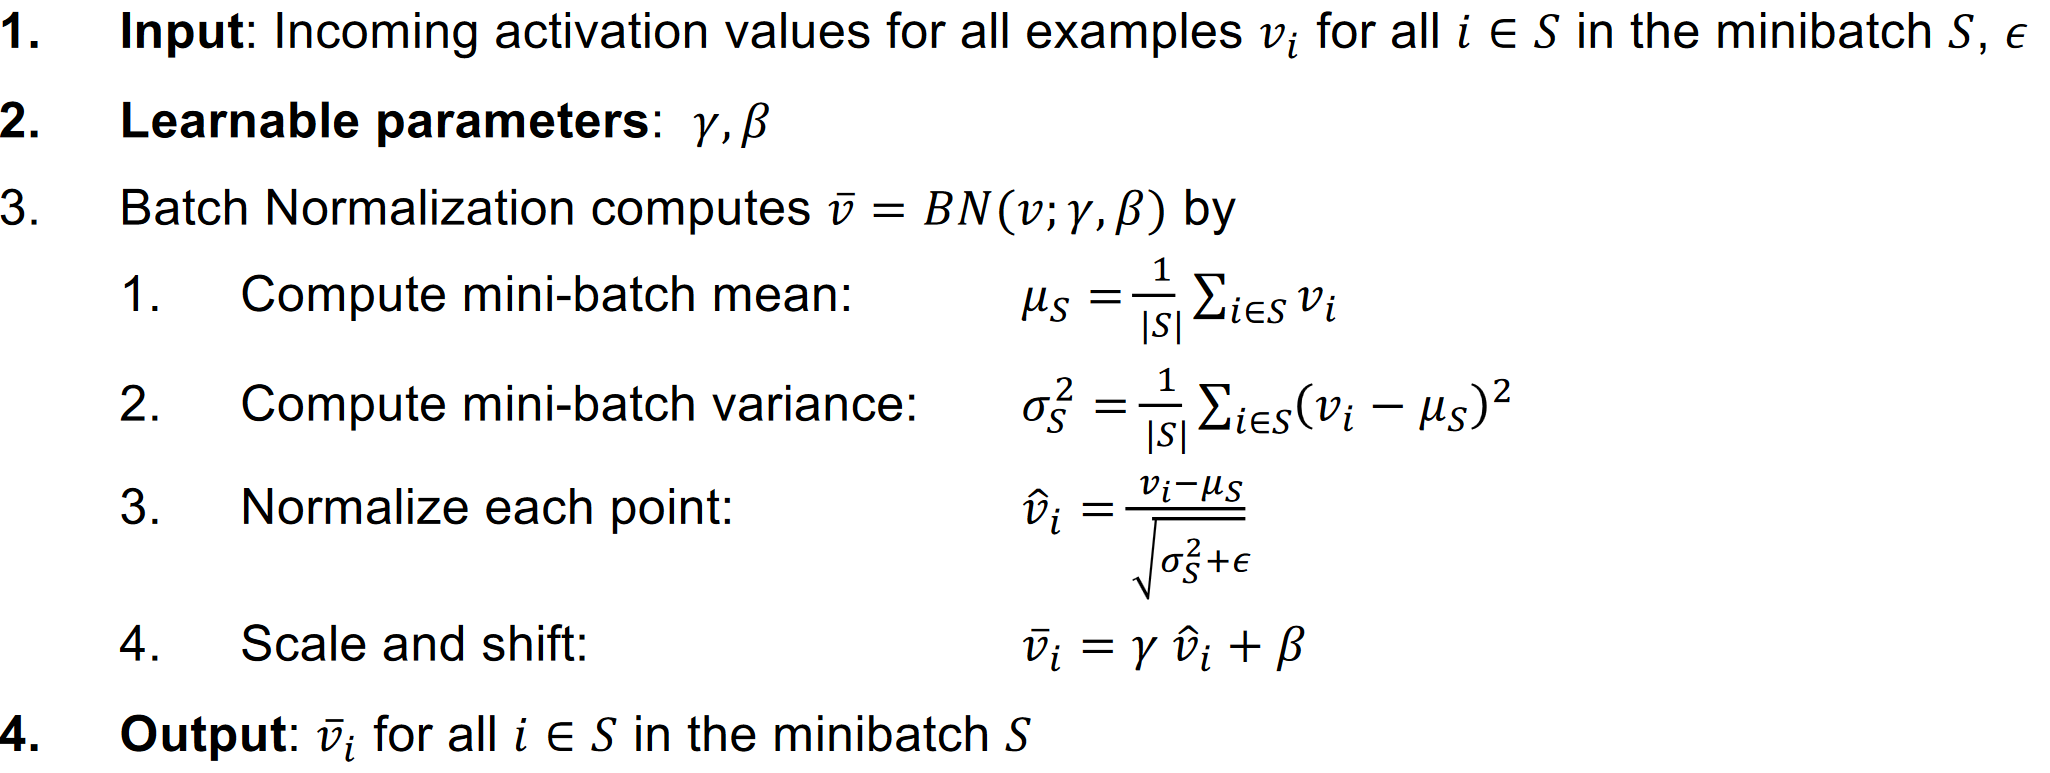
\includegraphics[width=0.9\linewidth]{pics/figure10.PNG}
\textbf{Convolutions in 1D}: 
Given vector $w \in \mathbb{R}^k$ and $x \in \mathbb{R}^d$, convolution result: $z_i = \sum^{min(i,k)}_{j = max(1, i-d+1)}{w_j}x_{i-j+1}$ \\
\textbf{Output}:
m $f\times f$ filters, a $n \times n$ image as input, padding p and stride s: output size = $\frac{n+2p-f}{s}+1$\\
\textbf{Pooling layers}:
aggregate several units (max/average) to decrease the width of the width of the network\\
\textbf{Residual Connections}
1. Skip connections for effectively training deeper networks;\quad 2. Allows identity as optimal solution (avoid vanishing gradients)
%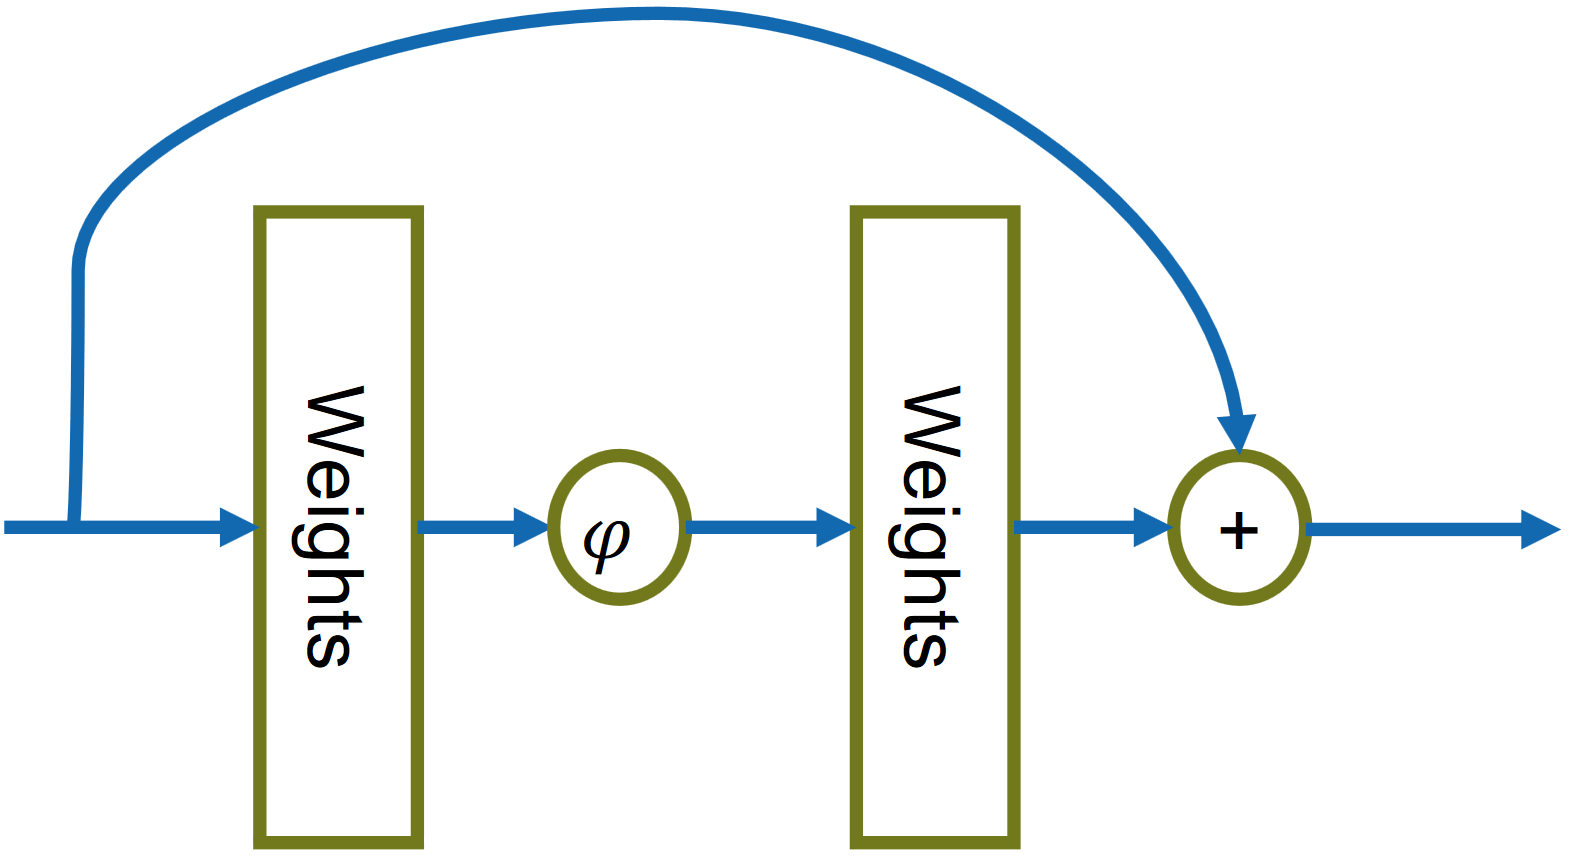
\includegraphics[width=\linewidth]{pics/figure11.PNG}


\section{Clustering (unsup. classification)}
    \textbf{K-Means problem:} Non-convex Opt. + NP hard\\
    Pick centers to minimize sum of squared distances: $\hat{R}(\mu) = \hat{R}(\mu_1, \cdots, \mu_k) = \sum_{i = 1}^{n} \mathrm{min}_{j \in \{ 1 \cdots k \} } \|x_i - \mu_j \|_2^2$
    
    \textbf{Lloyd’s heuristic:} 
    1.Initialize Cluster center 1...k\\
    2.While not converged: Assign points to closest center and update center with mean of its points \\
    \textbf{Properties}:
    Guaranteed to converge (to a local optimum); Sensitive to initialization; Number of iterations required can be exponential; Determining k is difficult; Cannot well model clusters of arbitrary shape
    
    \textbf{K-Means++}  
    % \hangindent=0.5cm
    1. Choose the first centroid $\mu$ uniformly rand. from X 
    2. For each $x \in X$ compute $D(x) := \mathrm{min}_j \|x - \mu_j \|_2^2$ 
    3. Sample the next $\mu_j$ from $X$ with probability $P(\mu_j = x) \propto D(x)^2$ 
    4. Repeat the last two steps until k centroids are chosen\\
    (Expected cost is $\mathcal{O}(log k)$ times that of optimal k-Means solution $\hat{R}(\mu_{++}) \leq \mathcal{O}(log k) \mathrm{min}_\mu \hat{R}(\mu)$)

    \textbf{Kernelized k-means} 
    k-means algorithm is kernelizable (objective only depends on $XX^T$); can use appropriate features $\phi(x)$ to cluster non-spherical and non-linearly separable clusters using k-means.
    
    

\section{Dimension reduction (unsup. reg)}
    \textbf{PCA:} Compress data with low dim. representation\\
    $(\boldsymbol{w}^*,\boldsymbol{z}^*)={\underset{||\boldsymbol{w}||^2_2=1,\boldsymbol{z}}{\mathrm{argmin}}} \sum_{i=1}^n ||z_i\boldsymbol{w}-\boldsymbol{x}_i||^2_2 $, 
    $z_i^*=\boldsymbol{w}^T\boldsymbol{x}_i$, 
    $\boldsymbol{w}^*=\underset{||\boldsymbol{w}||^2_2=1}{\mathrm{argmin}}\ \sum_{i=1}^n ||\boldsymbol{ww}^T\boldsymbol{x}_i - \boldsymbol{x}_i||^2$
    $=\underset{||\boldsymbol{w}||^2_2=1}{\mathrm{argmax}} \sum_i^{n} (\boldsymbol{w}^T \boldsymbol{x}_i) ^2$\quad if $\boldsymbol{w}$ is a 1-D vector.(k=1)\\

    
    $(\boldsymbol{W},\boldsymbol{z}_1,...,\boldsymbol{z}_n)=\underset{\boldsymbol{W}^T\boldsymbol{W}=\boldsymbol{I}_k,\boldsymbol{z}}{\mathrm{argmin}} \sum_i^n ||\boldsymbol{Wz}_i-\boldsymbol{x}_i||^2_2 $\\
    with orthogonal $\boldsymbol{W} = [\boldsymbol{v}_1| ... | \boldsymbol{v}_k] \in \mathbb{R}^{d \times k}$ and $\boldsymbol{z}_i = \boldsymbol{W}^T\boldsymbol{x}_i$ where $\boldsymbol{v}_{1...k}$ are the first k columns of $\boldsymbol{V}\ (SVD: \boldsymbol{X}= \boldsymbol{USV}^T)$\\
    \textit{Empirical Covariance:} $\boldsymbol{\Sigma} = \frac{1}{n}\sum_i \boldsymbol{x}_i\boldsymbol{x}_i^T $
    \makebox[0.5cm][]{}with Eigenvalues $\lambda_1\geq \lambda_2 \geq ... \Rightarrow$ $\boldsymbol{\Sigma} = \sum_i \lambda_i \boldsymbol{v}_i\boldsymbol{v}_i^T$ \\
    $\frac{1}{n}\underset{\boldsymbol{W}^T\boldsymbol{W}=\boldsymbol{I}_k}{\mathrm{argmin}} \sum ||\boldsymbol{Wz}_i-\boldsymbol{x}_i||^2_2 = \sum_{i=k+1}^d \lambda_i$
    
    \textbf{Kernel PCA:} $w = \sum_{j=1}^n {\alpha}^{(j)} \phi(x_j)$\\
    \centerline{$\boldsymbol{\alpha}^*= \underset{\boldsymbol{\alpha}^T\boldsymbol{K\alpha}=1}{\mathrm{argmax}}\; \boldsymbol{\alpha}^T\boldsymbol{K}^T\boldsymbol{K}\boldsymbol{\alpha} = \underset{\boldsymbol{\alpha}}{\mathrm{argmax}} \frac{\boldsymbol{\alpha}^T\boldsymbol{K}^T\boldsymbol{K}\boldsymbol{\alpha}}{\boldsymbol{\alpha}^T\boldsymbol{K}\boldsymbol{\alpha}}$}
    with solution $\alpha^{(i)} = \frac{1}{\sqrt{\lambda_i}}v_i$ from $K=\sum \lambda_iv_iv_i^T$\\
    A new point x is projected by: $z_i = \sum_{j=1:n} \alpha_j^{(i)} k(x_j,x)$
    
    \textbf{Autoencoders} initialization matters\\ 
    $f(x,\theta)=f_{dec}(f_{enc}(x;\theta_{enc});\theta_{dec})\quad \mathbb{R}^{d}\to \mathbb{R}^{k<d} \to \mathbb{R}^{d}$
    If linear activ. func., AE (non-conv.) equivalent to PCA.



\section{Statistical perspective}
\subsection{Estimate data distribution}
    \textbf{Generalization:}\\
    Assume data is generated iid. Goal: identify a hypothesis $f: X \rightarrow Y$ that minimized \textbf{expected loss} (\textbf{prediction error}, \textbf{population risk}) :
    $R(f) = \int p(x,y)  \ell(y; f(x))dxdy = \mathbb{E}_{x, y}[\ell(y, f(x))]$ \\
    \textbf{Empirical risk:} 
    $\hat{R}_D(f) = \frac{1}{|D|} \sum\limits_{(x, y) \in D} \ell(y; f(x)) $ \\
    \textbf{Generalization error:} 
    $| \hat{R}_D(f) - R(f) |  \rightarrow 0, |D| \rightarrow \infty$ 

    Traing data $D$, test data $D'$ from the same distribution:\\
    Solution: $\hat{f}_D = \underset {f \in F} { \operatorname {arg\,min} } \,  \hat{R}_D(f)$ \\
    Evaluation: $\hat{R}_{D'}(\hat{f}_D) = \frac{1}{|D'|} \sum\limits_{(x, y) \in D'} \ell(y, \hat{f}_D(x)) $ \\
    Obtain an overly optimistic estimate: $\mathbb{E}_{D}[\hat{R}_D(\hat{f}_D)] <= \mathbb{E}_{D}[R_D(\hat{f}_D)]$ (biased if no test)\\
    $\mathbb{E}_{D'}[\hat{R}_{D'}(\hat{f}_D)] = R(\hat{f}_D)$ (unbiased with test)

\subsection{ Regression}
    \textbf{Optimal predictor for the squared loss:}\\
    $f^*(x) =  \underset {f: X \rightarrow \mathbb{R}} { \operatorname {arg\,min} } \,  R(f)  =  \underset {f: X \rightarrow \mathbb{R}} { \operatorname {arg\,min} } \,  \mathbb{E}_{x, y}[\ell(y, f(x))]$ 

    \textbf{Bayes‘ optimal predictor for the squared loss:}
    $f^*(x) = \mathbb{E}[Y|X=x]$ 
    
    \textbf{Least-squares regression = Gaussian MLE:}
    Assume $y = f(x)+ \epsilon, \epsilon \sim \mathcal{N}(x;0,\sigma^2)$, $f(x)=w^Tx$,  $p(y|x) = \mathcal{N}(y;w^Tx,\sigma^2)$, 
    $\hat{w}_{MLE}= \mathrm{argmax}_w\; p(y_{1:n}|x_{1:n}, w^Tx,\sigma^2) =  \mathrm{argmin}_w\; -\sum_{i=1}^n \mathrm{log}\left[ P(y_i|x_i;w^Tx,\sigma^2)\right] = \mathrm{argmin}_w\; n/2 log(2 \pi \sigma^2) + \sum_{i=1}^n (y_i - w^T x_i)^2 / (2 \sigma^2)$\\

    \textbf{Ridge regression = Gaussian MAP estimation:}
    Assume noise $p(y|x, w)$ is iid Gaussian, $w \sim \mathcal{N}(0, \beta^2I)$
    $ \mathrm{argmax}_w\; p(w|D) =  \mathrm{argmax}_w\; p(w) \prod_{i=1}^n \mathrm{log}P(y_i|x_i;w)= \mathrm{argmin}_w\; \frac{1}{2\beta^2} \| w \|_2^2 + \frac{1}{2\sigma^2}\sum_{i=1}^n (y_i - w^T x_i)^2$

    \textbf{L1-regul.:} Laplace prior: $p(x; \mu, b) = \frac{1}{2b} exp(-\frac{|x - \mu|}{b})$
    
    \textbf{Student-t likelihood}: ${P(y|x, w, \nu, \sigma^2)={\frac {\Gamma ({\frac {\nu +1}{2}})}{{\sqrt {\nu \pi \sigma^2}}\,\Gamma ({\frac {\nu }{2}})}}\left(1+{\frac {
    (y-w^Tx)^{2}}{\nu \sigma^2}}\right)^{-\frac{(\nu +1)}{2}}}$
\subsection{ Classifier}
    \textbf{Population risk} with 0-1 loss:
    $R(f) = P(y \neq f(x)) = { \operatorname {arg\,min} } \,  \mathbb{E}_{x, y}[(y \neq f(x)]$

    \textbf{Bayes‘ optimal classifier: }
    $f^*(x) = { \operatorname {arg\,max} }_y \,p[Y=y|X=x]$ most probable class

    \textbf{Logistic regression = Bernoulli MLE:} $p(y|x) = Ber(y;\sigma(w^Tx))$ \\
    $\hat{w}_{MLE}= \mathrm{argmax}_w\; p(y_{1:n}|x_{1:n}, w^Tx,\sigma^2) =  \mathrm{argmin}_w\; -\sum_{i=1}^n \mathrm{log}\left[ P(y_i|x_i;w^Tx,\sigma^2)\right] = \mathrm{argmin}_w\; \sum_{i=1}^n log(1+exp(-y_iw^Tx_i))$\\
    Logistic loss is \textbf{convex}

    \textbf{Regularized logistic regression = Bernoulli MAP}
    L2 (Gaussian prior): $\mathrm{argmin}_w\; \sum_{i=1}^n log(1+exp(-y_iw^Tx_i)) + \lambda \|w \|_2^2$ \\
    L1 (Laplace prior): $\mathrm{argmin}_w\; \sum_{i=1}^n log(1+exp(-y_iw^Tx_i)) + \lambda \|w \|_1^2$ 

    \textbf{Classification:} $P(y|x, \hat{w}) = \frac{1}{1+exp(-y \hat{w}^Tx)}$
    
    \textbf{Multi-class logistic regression:} $P(y = i|x, \hat{w}_1, \cdots ,\hat{w}_c) = \frac{exp(\hat{w}_i^Tx)}{\sum_{j=1}^c exp(\hat{w}_j^Tx)}$

    \textbf{Cross-entropy loss:} $\ell (y, x;\hat{w}_1, \cdots ,\hat{w}_c) = -log(p(Y=y|, x, \hat{w}_1, \cdots ,\hat{w}_c))$ 

    \textbf{Kernelized logistic regression:} \\
    Learning: $\hat{\alpha} = \mathrm{argmin}_\alpha\; \sum_{i=1}^n log(1+exp(-y_i\alpha^TK_i)) + \lambda \alpha^T K \alpha$ \\
    Classification: $P(y|x, \hat{\alpha}) = \frac{1}{1+exp(-y \sum_{j=1}^n \hat{\alpha}_j^Tk(x_j, x)}$

\section{Bayesian decision theory}
    Given: \\
    1. Conditional distribution over labels $p(y|x)$ for $y \in Y$
    2. Set of actions $A$
    3. Cost function $C: Y \times A \rightarrow \mathbb{R}$ \\
    BDT: minimize the expected cost $a* = \mathrm{argmin}_{a \in A}\; \mathbb{E}_{y}[C(y, a)|x]$ \\

    
\subsection{ Regression: }
    Cond. dist: $p(y|x) = \mathcal{N}(x;f(x),\sigma^2)$, Act. set: $A = \mathbb{R}$, Cost func.: \\
    1. $C(y, a) = (y - a)^2$:  $a^*  =\mathbb{E}[y | x] = f(x)$ \\
    2. Asymmetric cost: $C(y, a) = c_1 \mathrm{max}(y-a, 0) +  c_2 \mathrm{max}(a-y, 0) $:  $a^* = f(x) + \Phi ^ {-1} (\frac{c_1}{c_1+c_2})$, CDF for Gaussian: $\Phi(z)$



\subsection{ Classification: }
    Cond. dist: $p(y|x) = Ber(y; \sigma (f(x)) )$, Act. set: $A = \{ +1, -1 \}$, Cost func.: \\
    1. $C(y, a) = [y \neq a]$:  $a^*  = \mathrm{argmax}_y\; p(y|x) = sign(f(x))$\\ \qquad $\mathbb{E}_{y}[C(y, a)|x] = 1 - p(y=a|x)$\\
    2. Asymmetric cost: 
    \vspace{-0.5cm}
        \begin{equation}
        C(y, a)=
        \begin{cases}
        c_{FP}& \text{y=-1, a=+1}\\
        c_{FN}& \text{y=+1, a=-1}\\
        0& \text{otherwise}
        \end{cases}
        \vspace{-0.2cm}
        \end{equation}
        $c_+ = \mathbb{E}_y[C(y, +1)|x]  = (1-p) \cdot c_{FP}$, $p = p(y=+1|x)$
        $c_- = \mathbb{E}_y[C(y, -1)|x]  = p \cdot c_{FN}$
        $a^* = 1: c+ <= c_{-} \Rightarrow p >= \frac{C_{FP}}{C_{FP} + C_{FN}}$ \\
        $c_{FN} / c_{FP}$ increases, more points classified as pos, TPR FPR increase\\
    3. With abstention (doubtful l.r.): $A=\{ +1, -1 , D\}$, $c < 0.5$, Less $c$: more likely to choose $D$ (doubtful)
     \vspace{-0.3cm}
        \begin{equation}
        C(y, a)=
        \begin{cases}
         c_m [y \neq a]& a \in \{+1, -1\}\\
         c& a=D
        \end{cases}
        \vspace{-0.2cm}
        \end{equation}
        \begin{equation}
        \vspace{-0.3cm}
        a^*=
        \begin{cases}
         y& P(y|x) \geq 1-c / c_m\\
         D& p > c / c_m \, or \, p < 1 - c / c_m
        \end{cases}
        \end{equation}
    $c_+ = (1-p)c_m, c_- = pc_m, c_D = c$ \\
    \textbf{Active sampling:} minimize the number of labels; \textit{violates i.i.d. assumption}; get stuck with bad model
    
    \textbf{Uncertainty sampling:} Given: unlabeled examples $D_U = \{x_1, \cdots, x_n \}$, labled dataset $D_L = \{ \}$. For $t = 1, 2, 3, \cdots$ 
    Estimate $p(y|x)$ given current $D_L$\\
    Pick unlabled example that we are most uncertain about (highest entropy): $i_t \in \mathrm{argmin}_{x \in D_U} H(p(y|x))$\\
    Query label $y_{i_t}$ and set $D_L \leftarrow D_L \cup \{( x_{i_t}, y_{i_t} )\}$
    



\section{Generative Model}

    \textbf{Discriminative:} $p(y|x)$ 
    \textbf{Generative:} $p(x, y)$ \\
    Can derive condi. from joint distr., but not vice versa!

    \textbf{Generative models for classification:}\\
    1. $P(X,Y) = P(X)P(Y|X)$ \\ density over inputs, probabilistic classifier\\
    2. $P(X,Y) = P(Y)P(X|Y)$ \\ prior over classes, appearence for each class\\

\subsection{Bayes Classifier (supervised)}\

    % 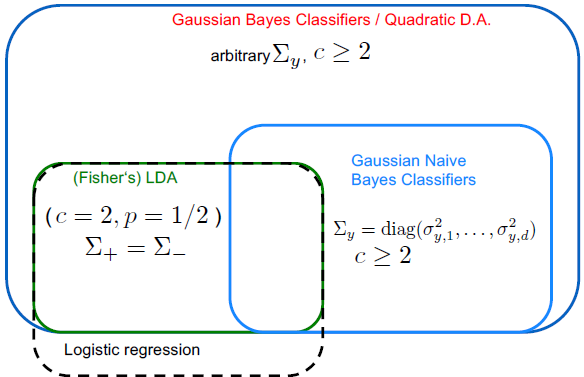
\includegraphics[width=0.5\linewidth]{pics/1.png}\\ % !改!!!!!!!!!!!!!!!!!!!!!!!

    \textbf{Naive Bayes Model:} 
    class prior: $P(Y=y) = p_y \, y \in \mathcal{Y} = \{1, \cdots , c \}$ \\
    features as conditionally independent given $Y$: $P(X_1, \cdots , X_d|Y) = \prod_{i=1}^d P(X_i|Y)$
    
    \textbf{Gaussian NBC:} \textbf{continuous} RV \\
    \textit{Learning:} 1. MLE: $P(Y=y) = \frac{Count(Y=y)}{n}$ \\ 
    2. MLE: $P(x_i|y) = \mathcal{N}(x_i|\mu_{y,i}, \sigma_{y,i}^2)$\\
    $\hat{\mu}_{y,i} = \frac{1}{Count(Y=y)} \sum_{j: y_j=y} x_{j,i}$
    $\sigma_{y,i}^2 = \frac{1}{Count(Y=y)} \sum_{j: y_j=y} (x_{j,i} - \hat{\mu}_{y,i})^2$\\
    \textit{Prediction:} $y = \mathrm{argmax}_{y'}\, P(y'|x) = \mathrm{argmax}_{y'}\, P(y')\prod_{i=1}^d P(X_i|Y)$

    \textbf{Categorical NBC:} \textbf{discrete} RV \\
    \textit{Learning:} 1. MLE: $P(Y=y) = \frac{Count(Y=y)}{n}$ \\ 
    2. MLE: $P(X_i = x|Y = y) = \theta_{x|y}^{(i)} = \frac{Count(X_i = x, Y = y)}{Count(Y = y)}$\\
    \textit{Prediction:} $y = \mathrm{argmax}_{y'}\, P(y'|x) = \mathrm{argmax}_{y'}\, P(y')\prod_{i=1}^d P(X_i|Y)$

    \textbf{Decision rules for binary classification:} Goal: $y = \mathrm{argmax}_{y'} P(y'|x) \Rightarrow y = sign(\mathrm{log} \frac{P(Y=1|x)}{P(Y=-1|x)})$

    \textbf{GNB, c=2, shared variance (= logistic regression = linear classifier):} \textit{discriminant function:} $f(x)=\mathrm{log} \frac{P(Y=1|x)}{P(Y=-1|x)} = w^Tx + w_0$,
    $w_i = \frac{\mu_{+, i} - \mu_{-, i}}{\sigma_{i}^2}$
    $w_0 = \mathrm{log} \frac{\hat{p}_+}{1-\hat{p}_+} + \sum_{i=1}^d \frac{\hat{\mu}_{-, i}^2 - \hat{\mu}_{+, i}^2}{2\hat{\sigma}_i^2}$

    Class distri.: $P(Y=1|x) = \frac{1}{exp(-f(x))} = \sigma (w^Tx+w_0)$

    \textbf{GBC:}
    class prior: $y \in \mathcal{Y} = \{1, \cdots , c \}$, $P(Y=y) = p_y = \frac{Count(Y=y)}{n}$ \\
    features as generated by multivariate Gaussian: $P(x|y) = \mathcal{N}(x;\mu_{y}, \Sigma_{y})$, 
    $\hat{\mu}_{y} = \frac{1}{Count(Y=y)} \sum_{i: y_i=y} x_{i}$
    $\Sigma_{y} = \frac{1}{Count(Y=y)} \sum_{i: y_i=y} (x_{i} - \hat{\mu}_{y})(x_{i} - \hat{\mu}_{y})^T$\\

    \textbf{Fisher's LDA:} $y = sign(f(x)) = sign(\boldsymbol{w}^T\boldsymbol{x} + w_0)$, $\boldsymbol{w} = \hat{\Sigma}^{-1} (\hat{\mu}_+ - \hat{\mu}_-)$, $w_0 = \frac{1}{2} (\hat{\mu}_-^T \Sigma^{-1} \hat{\mu}_- - \hat{\mu}_+^T \Sigma^{-1} \hat{\mu}_+)$

    \textbf{Conjugate priors:} \\
    Prior / Posterior \qquad Likelihood function\\
    Beta \qquad \qquad \qquad Bernoulli/Binomial\\
    Dirichlet \qquad \qquad Categorical/Multinomial\\
    Gaussian (fixed covariance) \qquad  Gaussian\\
    Gaussian-inverse Wishart \qquad  Gaussian\\
    Gaussian process \qquad  \qquad Gaussian\\


 \subsection{Gaussian Mixture Model (unsup.)}
    \textbf{Gaussian Mixture:} $P(x|\theta) = \sum_{y \in \{1, \cdots, i\ \cdots \}} \underbrace{w_i}_{p(y=i|\theta)}\cdot\underbrace{\mathcal{N}(x;\mu_i,\Sigma_i)}_{p(x|y=i,\theta)}$
    \vspace{-0.3cm}
    
    \textbf{Hard-EM Algorithm:}
    
    E-Step: Predict most likely class for each data point:\\
    $y_i^{(t)}=\mathrm{argmax}_yP(y|x_i,\theta^{(t-1)})=\mathrm{argmax}_y P(y|\theta^{(t-1)}) P(x_i|y,\theta^{(t-1)})$\\
    M-step: Compute MLE for GBC (closed form):\\
    \centerline{$\theta^{(t)}= \mathrm{argmax}_\theta P(D^{(t)}|\theta)$}
    Problem: Hard EM assigns a fixed label for uncertain x, even though the model is uncertain.\\
    Work poorly if clusters are \textbf{overlapping}
    
    \textbf{Soft EM:} \textit{\small(or just EM)}\\
    E-Step: Get cluster Membership with $\scriptstyle\mu^{(t-1)},\Sigma^{(t-1)},w^{(t-1)}$.\\
    \centerline{$\gamma_j(x) = P(y = j| x,\Sigma,\mu,w)= \frac{w_jP(x|\Sigma_j,\mu_j)}{\sum_l w_l P(x|\Sigma_l,\mu_l)}$}
    M-Step: Fit Clusters to weighted data points.\\
    \centerline{$w_j^{(t)}= \frac{1}{n}\sum_i\gamma_j^{(t)}(x_i);\;\mu_j^{(t)} = \frac{\sum_i\gamma_j^{(t)}(x_i)x_i}{\sum_i\gamma_j^{(t)}(x_i)}$}
    \centerline{$\Sigma_j^{(t)}= \frac{\sum_i\gamma_j^{(t)}(x_i)(x_i-\mu_j^{(t)})(x_i-\mu_j^{(t)})^T}{\sum_i \gamma_j^{(t)}(x_i)}$}

    \textbf{Initialization:} \textit{Weights:} typically uniform distr.; \textit{Means:} randomly initi./k-means++; \textit{Variances:} Spherical: $\Sigma_i = \sigma_i^2 I_d$, Diagonal: $\Sigma_i = diag(\sigma_1 = \cdots = \sigma_d)$, Tied: $\Sigma_1 = \cdots = \Sigma_k$
    
    \textbf{Degeneracy of GMM}: For \#Clusters = \#points the GMM overfits to $\mu=x$, $\sigma=0$. $\Rightarrow \text{ add } +\nu^2\mathbb{I}$ to the $\Sigma_j^{(t)}$ update.\\
    For semi-supervised GMM: Set $\gamma_j^{(t)}(x_i)= \mathbb m{1}_{\{j=y_i\}}$ for labeled data\\
    To select k=\#gaussians we can use cross-validation

    \textbf{Reasons mixture model useful:} 
    1. Can encode assumptions about “shape” of clusters 
    2. Can be part of more complex statistical models E.g., classifiers
    3. Probabilistic models can output likelihood $P(x)$ of a point $x$. (Useful for \textit{anomaly/outlier detection})
    4. Can be naturally used for semi-supervised learning
    
    \textbf{EM vs k-means}\\\hangindent=0.5cm
    K-Means equals to Hard-EM with equal weights \\
    $w=P(y|\theta)=\frac{1}{k}$ and spherical Variance $\Sigma_{1:k}=\sigma^2\mathbb{I}$
    
    \smallskip
    \textbf{General Expectation Maximation:}\\
    E-Step: $Q(\theta;\theta^{(t-1)})= \mathbb{E}_{z_{1:n}}\left[\mathrm{log} P(x_{1:n},z_{1:n}|\theta)| x_{1:n},\theta^{(t-1)}\right]$\\
    $=\sum_i\sum_{z_i}\gamma_{z_i}(x_i)\mathrm{log}P(z_i|\theta)P(x_i|z_i,\theta)$\\
    which equals to computing $\gamma_z(x_i)=P(z|x,\theta^{(t-1)})$
    
    M-Step: $\theta^{(t)}= \mathrm{arg max}_\theta\; Q(\theta;\theta^{(t-1)})$


\section{GANS}
    \centerline{$\underset{w_G}{\mathrm{min}} \;\underset{w_D}{\mathrm{max}} \underbrace{\mathbb{E}_x\mathrm{log}D(x;w_D)}_{\text{real images}}+\underbrace{\mathbb{E}_y\mathrm{log}\left[1-D(G(y;w_G);w_D)\right]}_{\text{fake images}}$}
    For a fixed generator $G$ the optimal discriminator $D$ is: \centerline{$D_G^*(x) = \frac{P_{data}(x)}{P_G(x)+P_{data}(x)}$}
    
    Simultanous gradient descent: Find saddle point\\
    \centerline{$w_G^{(t+1)}= w_G^{(t)}-\eta_t\nabla_{w_G}M(w_G,w_D^{(t)})$}
    \centerline{$w_D^{(t+1)}= w_D^{(t)}+\eta_t\nabla_{w_D}M(w_G^{(t)},w_D)$}
    
    Duality Gap: $DG = \underset{w_D'}{\mathrm{max}}M(w_G,w_D')-\underset{w_G'}{\mathrm{min}}M(w_G',w_D)$\\
    $DG = 0$ if $w_G, w_D$ form a pure equilibrium, else\,$DG > 0$



\section{Utilities}
    $\nabla_x x^TA = A \qquad \nabla_xa^Tx = \nabla_x x^Ta = a$
    
    $\nabla_x b^TAx = A^Tb \qquad \nabla_xx^Tx = 2x \qquad \nabla_x x^TAx = 2Ax$

    $Y=XW$: $\frac{\partial L}{\partial X} = \frac{\partial L}{\partial Y}W^T$, $\frac{\partial L}{\partial W} = X^T\frac{\partial L}{\partial W}$
    
    Bayes: $P(y|x)= \frac{P(x|y)P(y)}{P(x)}$ $Var(x) = \mathbb{E}[X^2] - \mathbb{E}[X]^2$
    
    Complexity ($X\in \mathbb{R}^{n\times d}$):\\\hangindent=0.5cm $X^TX \to \mathcal{O}(nd^2); \; X^{-1} \to \mathcal{O}(d^3);\; X^Ty \to  \mathcal{O}(nd)$ 

    Orthogonal matrix: $W^TW=I_k$; Trace: $tr(A) = tr(A^T)$

    $X \sim \mathcal{N}(0, I_d), Y = AX + \mu \sim \mathcal{N}(\mu, AA^T) $

    Maximum (conditional) likelihood estimation(\textbf{MLE}):\\
    $\theta^* = \mathrm{argmax}_\theta
    \hat{p}(y_1,\dots,y_n|\boldsymbol{x}_1,\dots,\boldsymbol{x}_n,\theta)$\\
    Maximum a posteriori estimate(\textbf{MAP}):\\
    \begin{tabular}{@{}c@{}}
    $p(w|\boldsymbol{x}_1,\dots,\boldsymbol{x}_n,y_1,\dots,y_n) = 
    \frac{p(w)p(y_1,\dots,y_n|\boldsymbol{x}_1,\dots,\boldsymbol{x}_n,w)}
    {p(y_1,\dots,y_n|\boldsymbol{x}_1,\dots,\boldsymbol{x}_n)}$
    \end{tabular}
   $f(x) = \frac{1}{\sigma\sqrt{2\pi}} \exp\left( -\frac{1}{2}\left(\frac{x-\mu}{\sigma}\right)^{\!2}\,\right)$
   ${\displaystyle f_{\mathbf {X} }(x_{1},\ldots ,x_{k})={\frac {\exp \left(-{\frac {1}{2}}({\mathbf {x} }-{\boldsymbol {\mu }})^{\mathrm {T} }{\boldsymbol {\Sigma }}^{-1}({\mathbf {x} }-{\boldsymbol {\mu }})\right)}{\sqrt {(2\pi )^{k}|{\boldsymbol {\Sigma }}|}}}}
$

Poisson: $P(x)=\frac{e^{-\lambda}\lambda^x}{x!}$, ${\displaystyle E(X)=V(X)=\lambda }$

Exponential: ${\displaystyle P(x;\lambda )= \lambda e^{-\lambda}}$, ${\displaystyle \operatorname {E} [X]={\frac {1}{\lambda }}}$, ${\displaystyle \operatorname {Var} [X]={\frac {1}{\lambda ^{2}}},}$

Bernoulli: ${\displaystyle f(k;p)=p^{k}(1-p)^{1-k}\quad {\text{for }}k\in \{0,1\}}$, ${\displaystyle \operatorname {E} \left(X\right)=p}$, $\operatorname {Var} [X]=pq=p(1-p)$

Binomial: ${\displaystyle f(k;n,p)=\Pr(X=k)={\binom {n}{k}}p^{k}(1-p)^{n-k}}$

Marginal: $P(z) = \sum_{x_i \in X} P(z, x_i)$
   

\end{multicols*}

\end{document}

